% ==============================================================================
% main.tex - ARQUIVO MESTRE ESTRUTURAL
% Ponto de entrada para compilação do artigo modular em formato IEEE Transactions
% ==============================================================================
\documentclass[journal, twocolumn]{IEEEtran}

% Inclusão das definições globais, pacotes e metadados
% ==============================================================================
% 00_config.tex - PREÂMBULO E CONFIGURAÇÕES GLOBAIS
% Artigo: A Contribuição de Federico Faggin para a Revolução dos Microprocessadores
%         e seus Impactos Sociais
% Padrão: IEEE Transactions (Two-Column Journal Format)
% ==============================================================================

% ------------------------------------------------------------------------------
% 1. CODIFICAÇÃO E SUPORTE A IDIOMA
% ------------------------------------------------------------------------------
\usepackage[utf8]{inputenc}               % Suporte à codificação UTF-8
\usepackage[T1]{fontenc}                  % Codificação de fontes de 8 bits
\usepackage[brazilian]{babel}             % Hifenização e termos em Português do Brasil

% Adequação de termos pré-definidos do IEEEtran para o Português
\renewcommand\IEEEkeywordsname{Palavras-Chave}
\addto\captionsbrazilian{%
  \renewcommand{\figurename}{Figura}%
  \renewcommand{\tablename}{Tabela}%
  \renewcommand{\refname}{Referências}%
  \renewcommand{\abstractname}{Resumo}%
}

% ------------------------------------------------------------------------------
% 2. PACOTES MATEMÁTICOS E FÍSICOS
% ------------------------------------------------------------------------------
\usepackage{amsmath, amssymb, amsfonts}  % Símbolos e ambientes matemáticos avançados
\usepackage{siunitx}                     % Unidades do SI e notação física padronizada
\sisetup{
  output-decimal-marker = {,},
  exponent-product = \cdot,
  per-mode = symbol,
  retain-explicit-plus = true
}

% ------------------------------------------------------------------------------
% 3. ELEMENTOS GRÁFICOS E TABELAS
% ------------------------------------------------------------------------------
\usepackage{graphicx}                    % Inclusão de figuras e diagramas
\graphicspath{{img/}}                    % Diretório padrão de imagens

\usepackage{booktabs}                    % Linhas tipográficas profissionais (\toprule, \midrule, \bottomrule)
\usepackage{tabularx}                    % Tabelas com largura controlada e quebra automática de parágrafo
\usepackage{array}                       % Formatação customizada de colunas
\usepackage{makecell}                    % Quebras de linha dentro de células
\usepackage{multirow}                    % Células de múltiplas linhas

% ------------------------------------------------------------------------------
% 4. CITAÇÕES, REFERÊNCIAS E TIPOGRAFIA
% ------------------------------------------------------------------------------
\usepackage{cite}                        % Compressão e ordenação de citações [1]-[3]
\usepackage{url}                         % Formatação de URLs
\usepackage{microtype}                   % Ajustes microtipográficos (evita overfull \hbox)

% Hiperlinks clicáveis sem caixas delimitadoras coloridas (estética clássica IEEE)
\usepackage[hidelinks]{hyperref}

% Referências cruzadas semânticas (cleveref) compatíveis com padrão brasileiro
\usepackage[nameinlink,noabbrev,brazilian]{cleveref}
\crefname{figure}{Figura}{Figuras}
\Crefname{figure}{Figura}{Figuras}
\crefname{table}{Tabela}{Tabelas}
\Crefname{table}{Tabela}{Tabelas}
\crefname{equation}{Equação}{Equações}
\Crefname{equation}{Equação}{Equações}
\crefname{section}{Seção}{Seções}
\Crefname{section}{Seção}{Seções}
\crefname{subsection}{Subseção}{Subseções}
\Crefname{subsection}{Subseção}{Subseções}

% ------------------------------------------------------------------------------
% 5. PARÂMETROS INSTITUCIONAIS E METADADOS
% ------------------------------------------------------------------------------
\def\universidade{Universidade Federal de Minas Gerais}
\def\siglauni{UFMG}
\def\faculdade{Escola de Engenharia}
\def\departamento{Departamento de Engenharia Elétrica}
\def\disciplina{Descobertas de Engenharia Elétrica que Moldaram a Sociedade Contemporânea}
\def\semestre{2º/2026}
\def\autorartigo{Luis Henrique Ribeiro Maciel}
\def\emailautor{luishrm@ufmg.br}

% Definição do Título e Cabeçalho do Artigo
\title{A Contribuição de Federico Faggin para a Revolução dos Microprocessadores e seus Impactos Sociais}

\author{\autorartigo%
% \thanks{Este trabalho faz parte da disciplina: \disciplina, oferecida no \semestre\ pelo \departamento\ da \universidade\ (\siglauni).}%
% \thanks{O autor é discente do curso de Engenharia Elétrica da \universidade\ (\siglauni), Av. Antônio Carlos, 6627, Pampulha, 31270-901, Belo Horizonte, MG, Brasil (e-mail: \emailautor).}%
}

% Cabeçalho de página IEEE (Running Header)
\markboth{UFMG -- DEE -- DESCOBERTAS DE ENGENHARIA ELÉTRICA}{}


\begin{document}

% Renderização do Título, Autoria e Notas Institucionais
\maketitle

% ------------------------------------------------------------------------------
% ELEMENTOS TEXTUAIS MODULARES
% ------------------------------------------------------------------------------
% Resumo e Palavras-Chave (Abstract e Keywords)
% ==============================================================================
% secoes/00_resumo.tex - RESUMO E PALAVRAS-CHAVE
% Tema: A Contribuição de Federico Faggin para a Revolução dos Microprocessadores
%       e seus Impactos Sociais
% ==============================================================================

\begin{abstract}

Este artigo analisa o papel de Federico Faggin no desenvolvimento do Intel 4004 (1971), o primeiro microprocessador comercial em pastilha única de silício, e seus desdobramentos tecnológicos e sociais. Examina-se como a implementação da tecnologia MOS com porta autoalinhada de silício (\textit{Silicon Gate Technology}, SGT) e as soluções de projeto de circuito e leiaute viabilizaram a integração de uma unidade central de processamento em um único circuito integrado. A metodologia emprega triangulação entre fontes primárias, modelagem analítica e registros orais dos projetistas. Os resultados evidenciam que a supressão das capacitâncias parasitas de sobreposição pelo SGT, aliada a contatos enterrados e cargas dinâmicas com \textit{bootstrapping}, proporcionou densidade e velocidade indispensáveis para a integração monolítica da CPU. Discutem-se os desdobramentos sociotécnicos dessa transição, que substituiu circuitos dedicados por processamento programável, fundou os sistemas embarcados e reestruturou a automação fabril.
\end{abstract}

\begin{IEEEkeywords}
Federico Faggin, Intel 4004, \textit{Silicon Gate Technology}, Microprocessadores, Sistemas VLSI, Impactos Sociais.
\end{IEEEkeywords}


% Seção I: Introdução (Contextualização do problema, objetivos e escopo)
% ==============================================================================
% secoes/01_introducao.tex - SEÇÃO I: INTRODUÇÃO
% Tema: Federico Faggin e o Primeiro Microprocessador Monolítico (Intel 4004)
% ==============================================================================

\section{Introdução}
\label{sec:introducao}

\IEEEPARstart{N}{o} final da década de 1960, o crescimento exponencial do número de conexões entre circuitos integrados de baixa e média escala de integração (SSI/MSI) encarecia os sistemas digitais e limitava a confiabilidade mecânica e elétrica das placas de circuito impresso. Esse cenário corresponde à chamada ``tirania dos números'' \cite{morton1958}: a complexidade de interconexão crescia mais rapidamente do que a capacidade de integrá-la com segurança, e a lei empírica de dobra da densidade de componentes \cite{moore1965} tornava a questão cada vez mais premente.

Nesse contexto, a fabricante japonesa de calculadoras Busicom contratou a Intel para conceber um conjunto de doze circuitos integrados customizados de função fixa. Em resposta, Marcian E. Hoff e Stanley Mazor propuseram uma arquitetura central programável por software, capaz de substituir a lógica dedicada por instruções armazenadas em memória. A proposta era conceitualmente viável, mas dependia de viabilização física: com a tecnologia MOS de porta de alumínio, a área requerida e as capacitâncias parasitas impediam a integração de uma CPU de uso geral em uma única pastilha economicamente viável \cite{faggin1996}.

Federico Faggin ingressou na Intel em 1970 para liderar o desenvolvimento físico e o projeto do conjunto MCS-4. Sua experiência prévia na criação e na industrialização da porta autoalinhada de silício (\textit{Silicon Gate Technology}, SGT) na Fairchild Semiconductor \cite{faggin1970} foi determinante para materializar a CPU em uma única pastilha de silício industrialmente viável \cite{faggin2021}.

O objetivo deste artigo é analisar as inovações em dispositivos semicondutores e as técnicas de layout concebidas por Faggin, relacionando a quebra de paradigmas técnicos às transformações econômicas e sociais decorrentes da difusão dos microprocessadores. Especificamente, busca-se: (i) analisar a transição da tecnologia MOS de porta metálica para o SGT; (ii) examinar as inovações de circuito, em particular as cargas ativas com \textit{bootstrapping} e o roteamento em dupla camada condutora; e (iii) avaliar as repercussões socioeconômicas, como o surgimento dos sistemas embarcados e da microcomputação.

O artigo está organizado como segue. A \cref{sec:fundamentacao} apresenta a fundamentação teórica de semicondutores; a \cref{sec:metodologia} descreve os métodos documentais adotados; a \cref{sec:resultados} expõe os resultados analíticos de projeto e os impactos na automação e na sociedade; a \cref{sec:discussao} discute os resultados e suas limitações; e a \cref{sec:conclusao} apresenta as conclusões.

% Seção II: Fundamentação Teórica (Física do SGT e família MCS-4)
% % ==============================================================================
% secoes/02_fundamentacao.tex - SEÇÃO II: FUNDAMENTAÇÃO TEÓRICA
% Tema: Federico Faggin e o Primeiro Microprocessador Monolítico (Intel 4004)
% ==============================================================================

\section{Fundamentação Teórica}
\label{sec:fundamentacao}

Conforme contextualizado na \cref{sec:introducao} e resumido nas \cref{fig:porta_mos_aluminio,fig:porta_mos_sgt}, a superação dos limites da porta metálica de alumínio exigiu reformular a geometria, a eletrostática e o projeto físico dos dispositivos PMOS \cite{cavin2012, mead1980}. Esta seção formaliza os modelos analíticos de capacitância parasita, atraso de comutação e tensão de limiar que quantificam o desempenho da tecnologia de porta autoalinhada de silício (SGT) \cite{faggin1970, sze2006}. Em seguida, examinam-se as soluções de circuito, as regras de \textit{layout} e a arquitetura de barramento multiplexado empregadas no conjunto MCS-4.

\subsection{Modelagem Física da Porta Metálica versus SGT}
\label{subsec:modelagem_fisica_sgt}

Em transistores MOS, o eletrodo de porta e o canal semicondutor atuam como placas condutoras paralelas de um capacitor separadas por uma lâmina isolante de dióxido de silício. A capacitância por unidade de área desse dielétrico ($C_{ox}$) varia na razão direta da permissividade do óxido ($\varepsilon_{ox} = \kappa_{ox}\varepsilon_0 \approx \SI{3,45e-11}{\farad\per\meter}$, produto da constante dielétrica adimensional do óxido $\kappa_{ox} \approx 3{,}9$ pela permissividade elétrica do vácuo $\varepsilon_0$) e na razão inversa da espessura física da película ($t_{ox}$):
\begin{equation}
\label{eq:cox}
C_{ox} = \frac{\varepsilon_{ox}}{t_{ox}}.
\end{equation}

A capacitância geométrica de sobreposição ($C_{ov}$) entre a porta e as difusões de fonte ou dreno decorre do produto de $C_{ox}$ pela área superposta:
\begin{equation}
\label{eq:cov}
C_{ov} = C_{ox} W L_{ov},
\end{equation}
em que $W$ indica a largura transversal do canal e $L_{ov}$ o comprimento longitudinal em que a porta recobre a região dopada adjacente. Na fabricação com porta de alumínio, em que a metalização ocorre após a formação de fonte e dreno, as tolerâncias de alinhamento das fotomáscaras acrescentam uma folga geométrica $\Delta L_{align}$ de \SIrange{3}{5}{\micro\meter} ao espalhamento térmico das impurezas:
\begin{equation}
\label{eq:lov_metal}
L_{ov,metal} = \Delta L_{align} + L_{diff,lat}.
\end{equation}
Nessa expressão, $L_{diff,lat} \approx 0{,}75 x_j$ representa a difusão lateral dos dopantes sob a borda da máscara, proporcional à profundidade vertical da junção ($x_j$) no substrato. Esse espalhamento lateral assemelha-se à tinta que avança ligeiramente sob a margem de uma fita protetora durante a aplicação. No processo SGT \cite{kerwin1969patent, faggin1970, klein1972patent}, o polissilício refratário é depositado antes das difusões. Como a própria porta atua como barreira de difusão, a folga litográfica anula-se ($\Delta L_{align} = 0$) e a sobreposição restringe-se à parcela lateral:
\begin{equation}
\label{eq:lov_sgt}
L_{ov,SGT} = L_{diff,lat}.
\end{equation}
Essa geometria (\cref{fig:modelo_capacitivo_geometria}) reduz $L_{ov}$ em três a cinco vezes e corta a capacitância parasita por borda entre 60\% e 80\% frente à porta metálica.

\begin{figure}[!t]
\centering
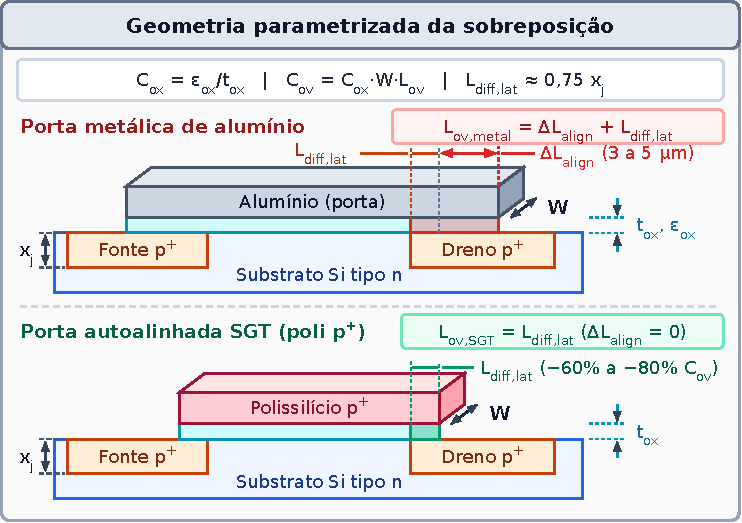
\includegraphics[width=\columnwidth]{modelo_capacitivo_geometria.pdf}
\caption{Geometria parametrizada da sobreposição entre porta metálica e SGT conforme as \cref{eq:cox,eq:cov,eq:lov_metal,eq:lov_sgt}, destacando $t_{ox}$, largura $W$, profundidade de junção $x_j$, difusão lateral $L_{diff,lat}$ e supressão da folga $\Delta L_{align} = 0$ na SGT.}
\label{fig:modelo_capacitivo_geometria}
\end{figure}

A redução de $C_{ov}$ atenua de forma amplificada a capacitância porta-dreno ($C_{gd}$) pelo efeito Miller durante a inversão lógica:
\begin{equation}
\label{eq:miller}
C_{in,Miller} = C_{gd} (1 - A_v) = C_{gd} (1 + |A_v|),
\end{equation}
em que $A_v = -g_m R_L$ é o ganho de tensão de pequenos sinais na região ativa, razão de amplificação entre saída e entrada cujo sinal negativo indica inversão de fase (sendo $g_m$ a transcondutância, isto é, a sensibilidade da corrente de saída em relação à tensão de porta, e $R_L$ a resistência efetiva de carga). Para módulos de ganho típicos $|A_v|$ entre 3 e 5, a capacitância física $C_{gd} \approx C_{ox} W L_{ov,d}$ (em que $L_{ov,d}$ representa a sobreposição junto ao dreno) é multiplicada por fatores de 4 a 6, penalizando o atraso de propagação ($\tau_{pd}$) da porta lógica \cite{weste2010}:
\begin{equation}
\label{eq:tau_pd}
\tau_{pd} \approx 0{,}69 R_{on} C_L \approx \frac{C_L \Delta V}{I_{on}},
\end{equation}
em que $R_{on}$ expressa a resistência equivalente do canal aberto em condução, $I_{on}$ a corrente útil fornecida para carregar ou descarregar o nó durante uma transição de amplitude $\Delta V$, e $C_L$ a capacitância total vista na saída:
\begin{equation}
\label{eq:cl_total}
C_L = C_{gd} (1 + |A_v|) + C_{gate,next} + C_{junc} + C_{wire}.
\end{equation}
Além do efeito Miller amplificado e das portas dos estágios seguintes ($C_{gate,next}$), a carga total incorpora as capacitâncias das junções $p\text{-}n$ reversamente polarizadas ($C_{junc}$, formadas na barreira entre as difusões $p^+$ e o substrato tipo $n$) e das trilhas metálicas de interconexão ($C_{wire}$). Esses dois termos operam como reservatórios secundários em paralelo que desviam parte da corrente $I_{on}$ destinada ao estágio subsequente. Ao contrair $C_{gd}$ e encurtar as ligações internas (\cref{fig:modelo_capacitivo_circuito}), o processo SGT reduziu $\tau_{pd}$ em até cinco vezes sob a mesma dissipação de potência.

\begin{figure}[!t]
\centering
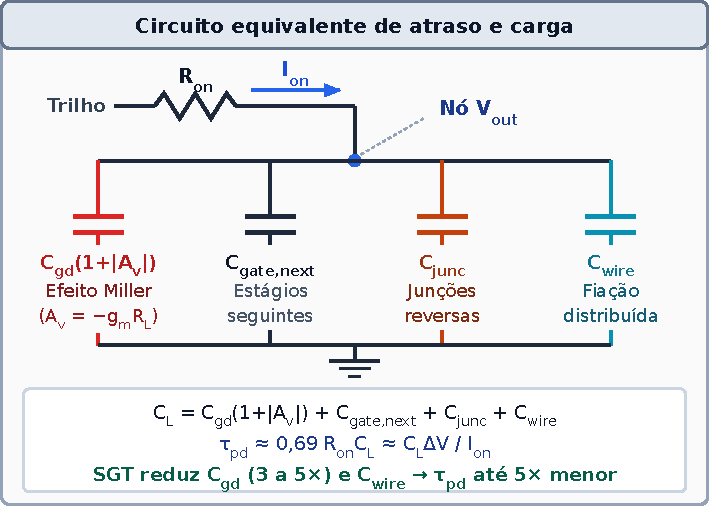
\includegraphics[width=\columnwidth]{modelo_capacitivo_circuito.pdf}
\caption{Circuito equivalente de carregamento do nó de saída conforme as \cref{eq:tau_pd,eq:cl_total}, relacionando $R_{on}$, $I_{on}$ e os quatro componentes de $C_L$.}
\label{fig:modelo_capacitivo_circuito}
\end{figure}

\subsection{Eletrostática da Tensão de Limiar e Propriedades Estruturais}
\label{subsec:eletrostatica_vth_estruturais}

A tensão de limiar ($V_{th}$) de um transistor PMOS em modo de enriquecimento (dispositivo normalmente desligado quando a tensão de porta é nula) sobre silício tipo $n$ decorre do equilíbrio eletrostático exigido para estabelecer o canal condutor:
\begin{equation}
\label{eq:vth_geral}
V_{th} = V_{FB} - 2\phi_F - \frac{Q_B}{C_{ox}}.
\end{equation}
A tensão de bandas planas ($V_{FB}$) representa o potencial inicial aplicado à porta apenas para compensar diferenças internas entre materiais e cargas presas no óxido antes de iniciar a atração de lacunas, de forma semelhante a tarar uma balança antes de medir a carga útil:
\begin{equation}
\label{eq:vfb}
V_{FB} = \Phi_{ms} - \frac{Q_{ss}}{C_{ox}},
\end{equation}
sendo $\Phi_{ms} = \Phi_m - \Phi_s$ a diferença de função de trabalho entre porta e substrato, e $Q_{ss}$ a densidade superficial de cargas fixas positivas na interface óxido-silício.

O potencial de Fermi ($\phi_F$), que quantifica o afastamento energético imposto pela dopagem do substrato em relação ao silício puro, e a densidade de carga espacial na zona de depleção ($Q_B$) são definidos por:
\begin{equation}
\label{eq:phi_f}
\phi_F = \frac{k T}{q} \ln\left(\frac{N_D}{n_i}\right),
\end{equation}
\begin{equation}
\label{eq:qb}
Q_B = \sqrt{2 q \varepsilon_{Si} N_D (2\phi_F + |V_{SB}|)},
\end{equation}
em que $kT/q$ é o potencial térmico (sendo $k$ a constante de Boltzmann e $T$ a temperatura absoluta), $N_D$ a concentração volumétrica de átomos doadores de elétrons no substrato tipo $n$, $n_i$ a concentração intrínseca de portadores no silício puro, $q$ a carga elementar e $\varepsilon_{Si}$ a permissividade do silício. A grandeza $Q_B$ corresponde à carga dos íons fixos exposta na faixa do substrato que precisa ser esvaziada de elétrons livres antes da chegada das lacunas do canal. Sob polarização de corpo ($V_{SB}$, tensão reversa entre fonte e substrato), essa zona esvaziada alarga-se e reforça a barreira à condução. A substituição de \cref{eq:vfb,eq:phi_f,eq:qb} em \cref{eq:vth_geral} resulta na forma expandida de $V_{th}$ para dispositivos PMOS:
\begin{equation}
\label{eq:vth_expandido}
V_{th} = \Phi_{ms} - \frac{Q_{ss}}{C_{ox}} - 2\phi_F - \frac{\sqrt{2 q \varepsilon_{Si} N_D (2\phi_F + |V_{SB}|)}}{C_{ox}}.
\end{equation}

A substituição do alumínio por silício policristalino com dopagem $p^+$ altera diretamente $\Phi_{ms}$. Na dopagem, a concentração de boro é tão elevada que o polissilício conduz de modo semelhante a um metal. O nível energético médio dos portadores desloca-se então para o topo da banda de valência, faixa ocupada por elétrons ligados na rede cristalina. Para alumínio sobre silício tipo $n$, com $\Phi_m \approx \SI{4,10}{\electronvolt}$ e $\Phi_s \approx \SI{4,31}{\electronvolt}$, tem-se $\Phi_{ms,Al} \approx \SI{-0,21}{\volt}$. No polissilício $p^+$, a função de trabalho soma a afinidade eletrônica ($\chi \approx \SI{4,05}{\electronvolt}$, energia liberada ao capturar um elétron livre no cristal) à largura de banda proibida ($E_g \approx \SI{1,12}{\electronvolt}$, intervalo energético entre as bandas de valência e condução). Resulta assim $\Phi_{poly(p^+)} \approx \chi + E_g \approx \SI{5,17}{\electronvolt}$, elevando a diferença para $\Phi_{ms,poly} \approx \SI{5,17}{\electronvolt} - \SI{4,31}{\electronvolt} \approx \SI{+0,86}{\volt}$. A diferença líquida entre os eletrodos vale:
\begin{equation}
\label{eq:delta_phims}
\begin{aligned}
\Delta \Phi_{ms} &= \Phi_{ms,poly} - \Phi_{ms,Al} \\
&\approx \SI{+0,86}{\volt} - (\SI{-0,21}{\volt}) \approx \SI{+1,07}{\volt}.
\end{aligned}
\end{equation}
Esse ganho positivo reduz a magnitude negativa de $V_{th}$ em cerca de \SI{1,1}{\volt}, deslocando tensões típicas próximas a \SI{-3,5}{\volt} para patamares em torno de \SI{-2,4}{\volt}.

A parcela $-Q_{ss}/C_{ox}$ mantém sinal negativo em canais $p$ porque as cargas interfaciais positivas repelem as lacunas. Na orientação cristalográfica $\langle 111 \rangle$, a maior densidade superficial de ligações atômicas incompletas impõe $Q_{ss}/q \approx \SIrange{4e11}{5e11}{\per\centi\meter\squared}$. Para um óxido de \SI{100}{\nano\meter} ($C_{ox} \approx \SI{34,5}{\nano\farad\per\centi\meter\squared}$), esse termo desloca $V_{th}$ em \SI{-1,9}{\volt} a \SI{-2,3}{\volt}, elevando $|V_{th}|$ para \SIrange{3,5}{5,0}{\volt}. Na orientação $\langle 100 \rangle$, a menor densidade atômica limita as cargas a $Q_{ss}/q \approx \SIrange{0,5e11}{1,0e11}{\per\centi\meter\squared}$, restringindo o deslocamento entre \SI{-0,2}{\volt} e \SI{-0,5}{\volt}. Combinando $\Phi_{ms}$, lâminas $\langle 100 \rangle$ e recozimentos em alta temperatura, o processo SGT estabilizou $V_{th}$ entre \SI{-1,5}{\volt} e \SI{-2,5}{\volt} \cite{faggin1970, klein1972patent}, permitindo alimentar o MCS-4 com $V_{SS} = \SI{+5}{\volt}$ e $V_{DD} = \SI{-10}{\volt}$ (\SI{15}{\volt} diferenciais) em compatibilidade direta com circuitos TTL no nível alto. A \cref{tab:comparacao_eletrica} sintetiza esses parâmetros eletrostáticos, cristalográficos e térmicos.

\begin{table}[!t]
\renewcommand{\arraystretch}{1.2}
\caption{Parâmetros Eletrostáticos, Cristalográficos e Térmicos entre Porta de Alumínio e SGT}
\label{tab:comparacao_eletrica}
\centering
\begin{tabularx}{\columnwidth}{>{\raggedright\arraybackslash}X >{\centering\arraybackslash}p{2.6cm} >{\centering\arraybackslash}p{2.6cm}}
\toprule
\textbf{Parâmetro} & \textbf{Porta de Alumínio} & \textbf{Porta SGT} \\
\midrule
Diferença $\Phi_{ms}$ & $\approx \SI{-0,21}{\volt}$ & $\approx \SI{+0,86}{\volt}$ \\
Orientação do silício & $\langle 111 \rangle$ & $\langle 100 \rangle$ \\
Cargas fixas ($Q_{ss}/q$) & \SIrange{4e11}{5e11}{\per\centi\meter\squared} & \SIrange{0,5e11}{1,0e11}{\per\centi\meter\squared} \\
Deslocamento ($-Q_{ss}/C_{ox}$) & \SIrange{-1,9}{-2,3}{\volt} & \SIrange{-0,2}{-0,5}{\volt} \\
Tensão de limiar ($V_{th}$) & \SIrange{-3,5}{-5,0}{\volt} & \SIrange{-1,5}{-2,5}{\volt} \\
Limite térmico do eletrodo & Fusão \SI{660}{\celsius} e eutético \SI{577}{\celsius} & Refratário ($> \SI{1100}{\celsius}$) \\
Excursão de saída ($V_{out}$) & $V_{DD} + |V_{th}|$ (atenuada) & $V_{DD}$ (plena com \textit{bootstrapping}) \\
\bottomrule
\end{tabularx}
\end{table}

Sob a óptica de materiais, o silício policristalino produzido por deposição química em fase de vapor (CVD, técnica em que gases reagentes depositam um filme sólido uniforme sobre a lâmina aquecida) permanece estável acima de \SI{1100}{\celsius}. Essa condição permite padronizar a porta antes das difusões de fonte e dreno, conduzidas entre \SI{1050}{\celsius} e \SI{1150}{\celsius}. Em contraste, o alumínio funde a \SI{660}{\celsius} e forma com o silício uma fase eutética líquida a apenas \SI{577}{\celsius}, temperatura na qual a mistura funde abaixo do ponto de fusão de ambos os elementos puros. Acima de \SI{450}{\celsius}, o silício solubiliza-se no metal ao longo de falhas lineares na grade atômica do cristal. No resfriamento, o alumínio preenche esses vazios formando espículas condutoras (\textit{spiking}) que perfuram junções rasas ($x_j \le \SI{2}{\micro\meter}$), de modo análogo à água que rompe uma barragem fina através de fissuras, inutilizando o dispositivo por fuga reversa.

A estabilidade térmica do polissilício viabilizou ainda a captura iônica com fósforo (\textit{phosphorus gettering}) em atmosfera de oxicloreto de fósforo ($\text{POCl}_3$) entre \SI{1000}{\celsius} e \SI{1050}{\celsius}. A película gerada de vidro de fosfossilicato (PSG) atua como esponja química que fixa íons móveis de sódio ($\text{Na}^+$), evitando derivas temporais em $V_{th}$ e reduzindo fugas de corrente. Adicionalmente, o polissilício depositado sobre o óxido espesso (camada isolante mais grossa usada fora dos transistores para isolar o substrato) funciona como segunda camada condutora independente. Em circuitos de camada metálica única, o cruzamento de sinais exigia túneis difusos $p^+$ no substrato, cuja resistência de folha (resistência elétrica medida entre lados opostos de qualquer quadrado da película) situava-se entre \SI{30}{\ohm} por quadrado e \SI{100}{\ohm} por quadrado, somada a elevada capacitância de junção e perda de área. O nível intermediário de polissilício sob o alumínio eliminou esses túneis.

\subsection{Inovações de Circuito e Metodologia de \textit{Layout} no Intel 4004}
\label{subsec:inovacoes_circuito_leiaute}

Para adaptar o processo SGT às conexões irregulares da lógica aleatória do Intel 4004, Faggin combinou três recursos físicos e circuitais: os contatos enterrados, as cargas ativas com \textit{bootstrapping} dinâmico e o roteamento ortogonal em duas camadas \cite{faggin1996, faggin2021}.

Os contatos enterrados (\textit{buried contacts}), iniciados experimentalmente na Fairchild e formalizados posteriormente na patente concedida a Leslie L. Vadasz \cite{vadasz1972patent, faggin1996, faggin2021}, substituem pontes metálicas locais por ligações diretas no silício. Antes da deposição do polissilício, janelas seletivas são abertas no óxido de porta nos pontos em que o filme policristalino deve tocar o substrato monocristalino. Na difusão térmica subsequente de boro, os dopantes migram pelo polissilício para o substrato subjacente, formando uma região $p^+$ contínua que estabelece uma junção ôhmica, isto é, uma ligação resistiva simétrica sem barreira retificadora de diodo. Em \textit{layouts} convencionais de camada única (\cref{fig:contatos_enterrados}), conectar uma porta ao dreno adjacente exigia duas aberturas verticais e uma ponte de alumínio sujeita a folgas de alinhamento. A remoção dessas ilhas metálicas reduziu em até 50\% a área das células de lógica aleatória, permitindo integrar \num{2300} transistores em \SI{12}{\milli\meter\squared} \cite{faggin1996, faggin2021}.

\begin{figure}[!t]
\centering
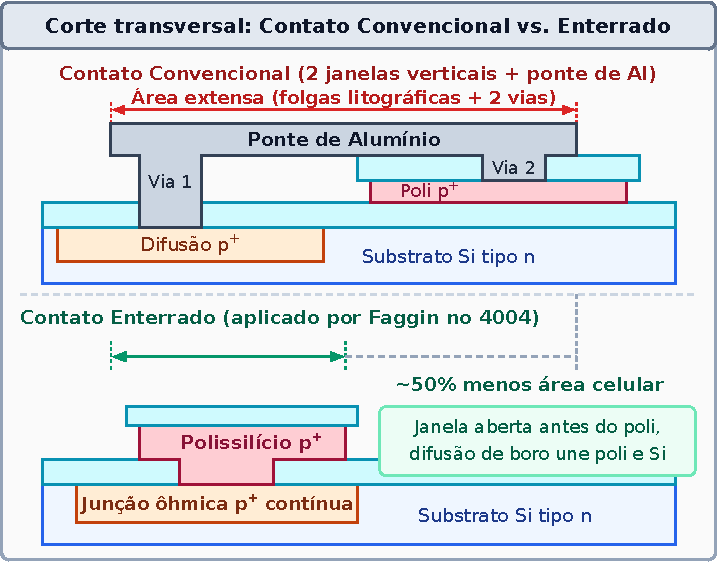
\includegraphics[width=\columnwidth]{contatos_enterrados.pdf}
\caption{Corte transversal comparando o contato convencional com duas janelas verticais e ponte de alumínio ao contato enterrado, cuja junção ôhmica $p^+$ contínua reduz cerca de 50\% da área celular.}
\label{fig:contatos_enterrados}
\end{figure}

No domínio dos circuitos, as cargas ativas com \textit{bootstrapping} dinâmico eliminaram a perda de excursão lógica inerente a inversores PMOS convencionais \cite{faggin1972fourchip, faggin1996}. No sistema MCS-4, o potencial de repouso é $V_{SS} = \SI{+5}{\volt}$ e a alimentação ativa é negativa ($V_{DD} = \SI{-10}{\volt}$). Na configuração convencional (\cref{fig:bootstrapping_circuito}), o transistor de entrada ($M_{in}$) liga a saída ($V_{out}$) a $V_{SS}$, enquanto o transistor de carga em enriquecimento ($M_{load}$) mantém dreno e porta fixos em $V_{DD}$, atuando $V_{out}$ como sua fonte. Quando $M_{in}$ corta, $M_{load}$ descarrega $V_{out}$ de \SI{+5}{\volt} em direção a \SI{-10}{\volt} enquanto $|V_{GS}| = V_{out} - V_{DD} > |V_{th}|$. À medida que $V_{out}$ desce, a tensão porta-fonte contrai até a condução cessar em:
\begin{equation}
\label{eq:vout_max_sem_boot}
V_{out,\text{lim}} = V_{DD} + |V_{th}|.
\end{equation}
Com $V_{DD} = \SI{-10}{\volt}$ e $|V_{th}| \approx \SI{2}{\volt}$, a saída estanca próxima a \SI{-8}{\volt}, ficando aquém de $V_{DD}$ por $|V_{th}|$, o que comprime a margem de ruído e retarda a cauda da transição.

\begin{figure}[!t]
\centering
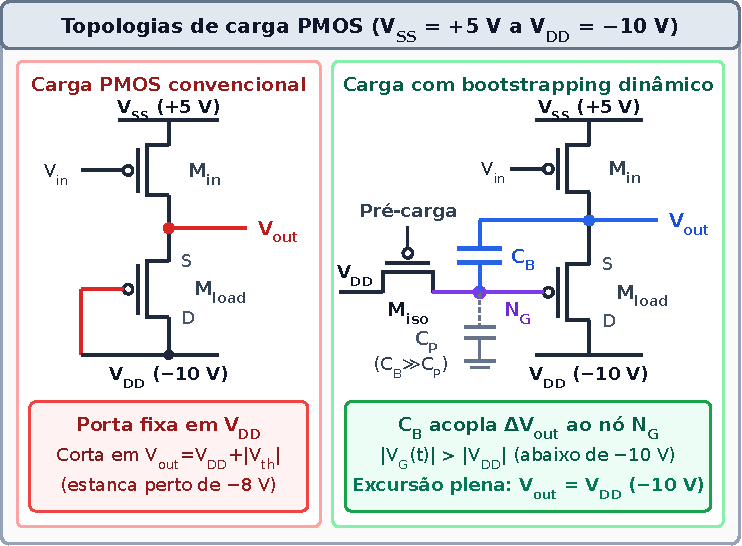
\includegraphics[width=\columnwidth]{bootstrapping_circuito.pdf}
\caption{Topologias de carga PMOS sob polaridade negativa ($V_{SS} = \SI{+5}{\volt}$ a $V_{DD} = \SI{-10}{\volt}$), comparando a carga convencional com porta fixa em $V_{DD}$ ao circuito com \textit{bootstrapping} dinâmico ($M_{iso}$, nó flutuante $N_G$, capacitor integrado $C_B$ e parasita $C_P \ll C_B$).}
\label{fig:bootstrapping_circuito}
\end{figure}

Para alcançar excursão integral até $V_{DD}$, o circuito com \textit{bootstrapping} associa um transistor de isolamento e amostragem ($M_{iso}$), a carga $M_{load}$ comandada por um nó flutuante em alta impedância ($N_G$, ponto isolado dos trilhos capaz de reter carga elétrica temporariamente) e um capacitor integrado ($C_B$) entre $V_{out}$ e $N_G$ (\cref{fig:bootstrapping_circuito}). Durante a pré-carga, etapa preparatória que fixa o estado inicial do nó, $M_{iso}$ conduz e carrega $N_G$ com uma tensão negativa $V_{G,inicial}$, entrando em corte logo após para isolar $N_G$. Quando $M_{in}$ bloqueia e $V_{out}$ sofre um degrau negativo $\Delta V_{out}$ em direção a $V_{DD}$, o capacitor $C_B$ acopla essa variação a $N_G$ por divisão capacitiva, à semelhança de uma plataforma que acompanha o deslocamento da saída, mantendo o transistor em condução até o fim do percurso:
\begin{equation}
\label{eq:delta_vg_boot}
\Delta V_G = \left( \frac{C_B}{C_B + C_P} \right) \Delta V_{out},
\end{equation}
em que $C_P$ reúne as capacitâncias parasitas em $N_G$. Dimensionando $C_B \gg C_P$, resulta $\Delta V_G \approx \Delta V_{out}$, de modo que a soma da pré-carga negativa com o degrau acoplado desloca $V_G(t)$ além de $V_{DD}$ em módulo:
\begin{equation}
\label{eq:vg_total_boot}
V_G(t) \approx V_{G,inicial} + \Delta V_{out}.
\end{equation}
Conforme mostra a \cref{fig:bootstrapping_ondas}, $V_G(t)$ mergulha abaixo de \SI{-10}{\volt}, preservando $|V_{GS}| > |V_{th}|$ durante toda a descarga. O transistor $M_{load}$ permanece na região de triodo, regime em que o canal conduz como resistor de baixa queda até igualar $V_{out} = V_{DD}$, restaurando a margem de ruído e acelerando a comutação \cite{faggin1972fourchip}.

\begin{figure}[!t]
\centering
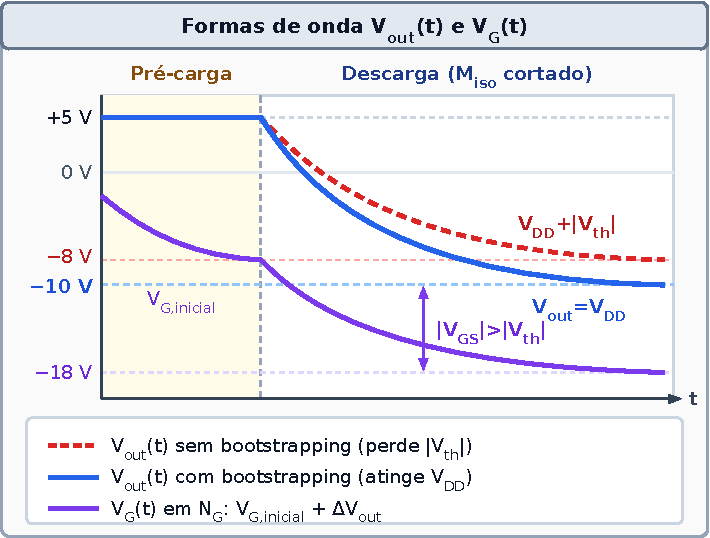
\includegraphics[width=\columnwidth]{bootstrapping_ondas.pdf}
\caption{Formas de onda $V_{out}(t)$ e $V_G(t)$, ilustrando a estagnação em $V_{DD} + |V_{th}|$ (\SI{-8}{\volt}) sem o estágio auxiliar e a excursão plena até $V_{DD}$ (\SI{-10}{\volt}) quando o degrau negativo em $C_B$ leva $V_G(t)$ abaixo de \SI{-10}{\volt}.}
\label{fig:bootstrapping_ondas}
\end{figure}

No traçado da pastilha, cujos blocos de controle, decodificadores e somadores carecem da regularidade de memórias, Faggin estabeleceu uma disciplina de roteamento ortogonal em duas camadas sem apoio de ferramentas automáticas de síntese (\cref{fig:roteamento_ortogonal}) \cite{faggin1996, faggin2021}. As pistas de polissilício $p^+$ foram orientadas no eixo vertical e as trilhas de alumínio no eixo horizontal perpendicular. As conexões entre esses dois níveis condutores utilizavam vias verticais, janelas abertas no óxido isolante intermediário para ligar o alumínio ao polissilício, enquanto os contatos enterrados uniam o polissilício às difusões do substrato. Essa regra geométrica evitou desvios, conteve o acoplamento capacitivo entre fios e reduziu a área de silício.

\begin{figure}[!t]
\centering
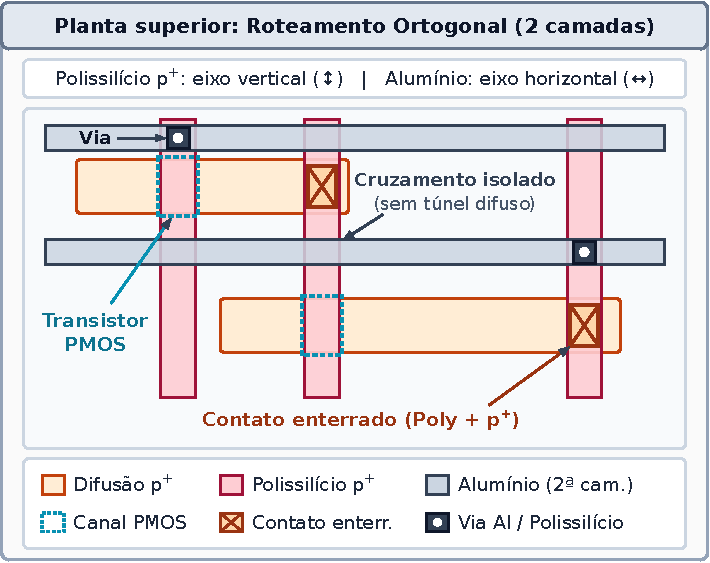
\includegraphics[width=\columnwidth]{roteamento_ortogonal.pdf}
\caption{Planta superior do roteamento ortogonal em duas camadas no Intel 4004, com trilhas verticais de polissilício $p^+$ e pistas horizontais de alumínio interligadas por vias verticais e contatos enterrados sem túneis difusos.}
\label{fig:roteamento_ortogonal}
\end{figure}

\subsection{Arquitetura do Sistema MCS-4 e Barramento Multiplexado}
\label{subsec:arquitetura_mcs4_barramento}

A família MCS-4 (\textit{Micro Computer Set}) implementa um computador modular em quatro circuitos integrados fabricados em PMOS SGT de \SI{10}{\micro\meter}, acondicionados em invólucros cerâmicos DIP de 16 pinos \cite{intel1971datasheet, intel1973mcs4, noyce1981}. O processador Intel 4004 reúne cerca de \num{2300} transistores em \SI{12}{\milli\meter\squared} e executa 46 instruções sob relógio bifásico. Seu núcleo integra uma unidade lógica e aritmética (ULA, bloco que efetua somas, subtrações e operações bit a bit) de 4 bits com correção para codificação decimal binária (BCD, formato que representa dígitos de 0 a 9 em grupos de 4 bits para calculadoras), um acumulador (registrador principal que armazena resultados intermediários), um indicador de transporte (\textit{carry}, sinalizador de transbordo gerado quando uma soma excede 4 bits), 16 registradores de índice de 4 bits (memória interna rápida endereçável em pares de 8 bits) e um contador de programa de 12 bits com pilha de três níveis (apontador de endereço da próxima instrução com três posições de retorno para sub-rotinas).

Os demais componentes fornecem memória e expansão de entrada e saída sobre o mesmo barramento (\cref{fig:mcs4_arquitetura_blocos}). O Intel 4001 incorpora \num{2048} bits de ROM mascarada (memória somente de leitura gravada permanentemente na fábrica durante a fotolitografia), dispostos em 256 palavras de 8 bits e uma porta de entrada e saída de 4 bits, admitindo até 16 unidades no sistema (4 quilobytes). O Intel 4002 provê \num{320} bits de RAM dinâmica (memória de leitura e escrita que retém dados em capacitores internos renovados periodicamente), distribuídos em quatro registradores de 20 caracteres de 4 bits com porta de saída e seleção por quatro linhas CM-RAM. O Intel 4003 atua como expansor estático de saída (circuito que amplia as linhas disponíveis mantendo os dados retidos) mediante um registrador de deslocamento de 10 bits, cadeia que recebe bits em série por um único fio e os disponibiliza simultaneamente em saídas paralelas para periféricos.

Em 1971, limites de custo e rendimento confinavam o encapsulamento comercial a 16 pinos, inviabilizando barramentos distintos para endereços, instruções e dados. Para contornar essa restrição, adotou-se um barramento bidirecional multiplexado no tempo de 4 bits ($D_0$ a $D_3$) \cite{intel1971datasheet, intel1973mcs4, faggin1974patent}. Os 16 terminais do Intel 4004 compreendem quatro pinos de dados ($D_0$ a $D_3$), duas entradas de relógio ($\phi_1$ e $\phi_2$), saída de sincronização (\textit{SYNC}), entradas de reinicialização (\textit{RESET}) e teste lógico (\textit{TEST}), quatro linhas de seleção de RAM (CM-RAM0 a CM-RAM3), habilitação de ROM (CM-ROM) e dois terminais de alimentação ($V_{SS} = \SI{+5}{\volt}$ e $V_{DD} = \SI{-10}{\volt}$).

\begin{figure}[!t]
\centering
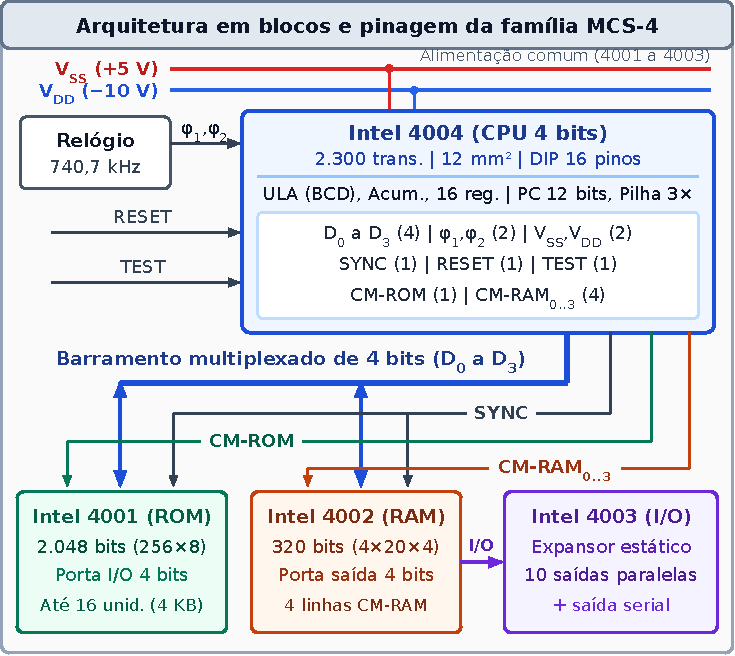
\includegraphics[width=\columnwidth]{mcs4_arquitetura_blocos.pdf}
\caption{Diagrama em blocos dos circuitos integrados 4004, 4001, 4002 e 4003 do sistema MCS-4, exibindo a pinagem de 16 pinos da CPU, o barramento bidirecional de 4 bits ($D_0$ a $D_3$), as linhas de controle e os trilhos $V_{SS} = \SI{+5}{\volt}$ e $V_{DD} = \SI{-10}{\volt}$.}
\label{fig:mcs4_arquitetura_blocos}
\end{figure}

O sincronismo baseia-se em um relógio bifásico ($\phi_1$ e $\phi_2$), composto por dois pulsos alternados que nunca permanecem ativos juntos, à semelhança das comportas de uma eclusa em que uma fecha antes de a outra abrir para evitar conflitos elétricos no barramento. Com período nominal de \SI{1,35}{\micro\second} (\SI{740,7}{\kilo\hertz}), uma instrução de uma palavra (8 bits) requer oito períodos de relógio, definindo um ciclo de \SI{10,8}{\micro\second} (aproximadamente \num{92600} instruções por segundo), enquanto instruções de duas palavras (16 bits) consomem \SI{21,6}{\micro\second} \cite{intel1971datasheet, intel1973mcs4}. Conforme ilustra a \cref{fig:mcs4_cronograma_subciclos}, o ciclo de \SI{10,8}{\micro\second} reparte-se em oito subciclos:
\begin{enumerate}
\item A1 (\textit{Address 1}): envio dos quatro bits menos significativos de endereço da ROM ($A_0$ a $A_3$).
\item A2 (\textit{Address 2}): envio dos quatro bits intermediários de endereço da ROM ($A_4$ a $A_7$).
\item A3 (\textit{Address 3}): envio dos quatro bits mais significativos de endereço da ROM ($A_8$ a $A_{11}$).
\item M1 (\textit{Memory 1}): leitura dos quatro bits superiores da instrução na ROM, código de operação (OPR).
\item M2 (\textit{Memory 2}): leitura dos quatro bits inferiores da instrução na ROM, modificador de operação (OPA).
\item X1 (\textit{Execute 1}): decodificação da instrução e início da execução lógica ou aritmética na ULA e registradores.
\item X2 (\textit{Execute 2}): conclusão das operações na ULA, atualização do acumulador e do indicador \textit{carry}, além do envio de endereço ou dado em operações com RAM e portas.
\item X3 (\textit{Execute 3}): conclusão do ciclo de execução, eventuais transferências de entrada ou saída com a RAM 4002 e emissão do pulso \textit{SYNC} para anunciar o ciclo seguinte.
\end{enumerate}

\begin{figure}[!t]
\centering
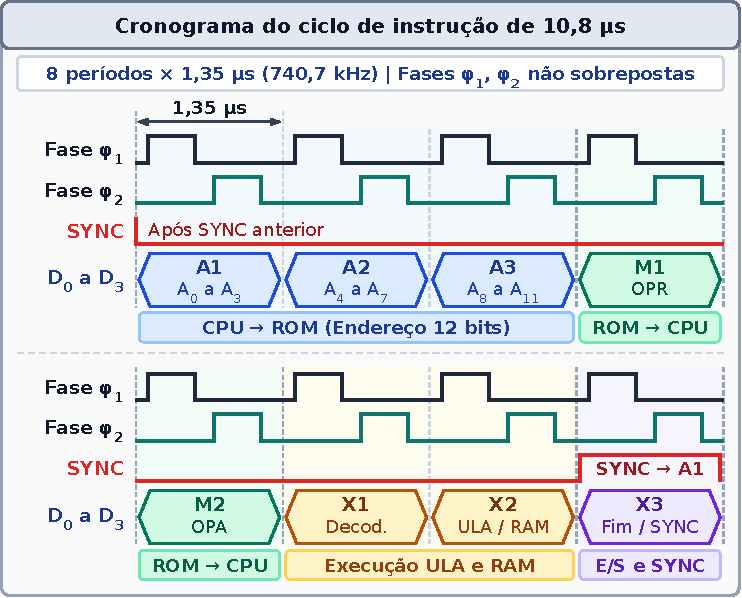
\includegraphics[width=\columnwidth]{mcs4_cronograma_subciclos.pdf}
\caption{Cronograma de \SI{10,8}{\micro\second} do sistema MCS-4 sob relógio bifásico não sobreposto ($\phi_1$, $\phi_2$ a \SI{740,7}{\kilo\hertz}), sinal $\text{SYNC}$ e os oito subciclos A1 a X3 divididos em duas faixas.}
\label{fig:mcs4_cronograma_subciclos}
\end{figure}


% % Seção III: Metodologia (Pesquisa histórica, técnica e documental)
% % ==============================================================================
% secoes/03_metodologia.tex - SEÇÃO III: METODOLOGIA
% Tema: Federico Faggin e o Primeiro Microprocessador Monolítico (Intel 4004)
% ==============================================================================

\section{Metodologia}
\label{sec:metodologia}

\subsection{Tipo de Estudo}
\label{subsec:metodologia_abordagem}

Trata-se de pesquisa histórica e analítica, de base técnica e documental, voltada à interface entre a física dos dispositivos semicondutores e a arquitetura de computadores.

\subsection{Fontes Primárias e Secundárias}
\label{subsec:metodologia_coleta}

As fontes primárias consistem em:
\begin{itemize}
\item patentes industriais de Federico Faggin sobre dispositivos MOS e métodos de fabricação com porta de silício, como a US Patent 3.475.234 \cite{faggin1969patent}, e a patente US 3.821.715 sobre o sistema de memória do computador multichip \cite{faggin1974patent};
\item manuais técnicos e notas de aplicação da Intel, em particular o \textit{MCS-4 Micro Computer Set Users Manual} \cite{intel1973mcs4};
\item documentos autobiográficos e artigos memoriais técnicos de Faggin sobre o desenvolvimento da arquitetura e das regras de layout do 4004 \cite{faggin1996, faggin2021}.
\end{itemize}

As fontes secundárias compreendem:
\begin{itemize}
\item periódicos especializados em história da tecnologia e dos semicondutores, como \textit{IEEE Micro} e \textit{Proceedings of the IEEE} \cite{noyce1981, cavin2012};
\item tratados clássicos de circuitos integrados e arquitetura de computadores \cite{mead1980, weste2010};
\item estudos socioeconômicos sobre automação industrial e difusão de tecnologias digitais nas últimas décadas do século XX.
\end{itemize}

\subsection{Procedimento de Análise}
\label{subsec:metodologia_triangulacao}

O procedimento consiste na triangulação sistemática entre três conjuntos de dados: (i) a física de dispositivos semicondutores; (ii) os parâmetros analíticos dos circuitos integrados, extraídos de patentes e manuais; e (iii) os relatórios históricos sobre a difusão industrial dos microprocessadores. As relações analíticas da \cref{sec:resultados} são tratadas como modelos de primeira ordem, usados para explicitar tendências, e não para reproduzir valores de projeto.


% % Seção IV: Resultados (Equações, tabelas e impactos industriais e sociais)
% % ==============================================================================
% secoes/04_resultados.tex - SEÇÃO IV: RESULTADOS
% Tema: Federico Faggin e o Primeiro Microprocessador Monolítico (Intel 4004)
% ==============================================================================

\section{Resultados}
\label{sec:resultados}

A viabilização física do Intel 4004 em uma única pastilha de silício resultou da convergência entre a tecnologia de porta autoalinhada de silício (SGT), técnicas de \textit{layout} compacto e circuitos dinâmicos de carga. Ao solucionar os entraves eletrostáticos e geométricos da lógica aleatória, Federico Faggin obteve métricas de velocidade e densidade que habilitaram a produção comercial do microprocessador e alteraram a organização da indústria eletrônica. Esta seção reúne os resultados quantitativos alcançados no dispositivo e no circuito, seguidos da análise de seus impactos industriais, econômicos e sociais.

\subsection{Inovações Técnicas de Dispositivo e Circuito}
\label{subsec:contribuicoes_tecnicas}

A aplicação das equações da \cref{subsec:modelagem_fisica_sgt} aos parâmetros nominais de fabricação do Intel 4004 ($t_{ox} \approx \SI{100}{\nano\meter}$ e $\kappa_{ox} \approx 3{,}9$) resulta em uma capacitância específica de óxido $C_{ox} \approx \SI{34,5}{\nano\farad\per\centi\meter\squared}$, equivalente a \SI{0,345}{\femto\farad\per\micro\meter\squared} (\cref{eq:cox}) \cite{faggin1970, sze2006}. Como a porta refratária de polissilício elimina a margem litográfica de alinhamento ($\Delta L_{align} = 0$, \cref{eq:lov_sgt}), a sobreposição longitudinal restringe-se à difusão lateral $L_{ov} \approx \SIrange{0,5}{1,0}{\micro\meter}$, contra \SIrange{3,5}{6,0}{\micro\meter} na porta de alumínio. Pela \cref{eq:cov}, essa redução comprime a capacitância de sobreposição $C_{ov}$ para a faixa de \SIrange{0,17}{0,35}{\femto\farad\per\micro\meter} de largura de canal, ante \SIrange{1,2}{2,1}{\femto\farad\per\micro\meter} no processo metálico. A queda resultante em $C_{gd}$ atenua o carregamento amplificado pelo efeito Miller (\cref{eq:miller}) e reduz o atraso de propagação $\tau_{pd}$ (\cref{eq:tau_pd}), elevando a frequência máxima de relógio em até cinco vezes sob a mesma litografia de \SI{10}{\micro\meter} \cite{faggin1970, faggin1996}.

No plano eletrostático (\cref{eq:vth_expandido,eq:delta_phims}), a combinação do polissilício $p^+$ com lâminas de orientação $\langle 100 \rangle$, cujos parâmetros constam da \cref{tab:comparacao_eletrica}, reduziu o módulo da tensão de limiar $V_{th}$ no Intel 4004 \cite{klein1972patent, sze2006}. Essa redução viabilizou a operação do conjunto MCS-4 com diferença de \SI{15}{\volt} entre trilhos, garantindo compatibilidade direta em nível alto com circuitos bipolares TTL sem conversores externos \cite{intel1971datasheet}. Em paralelo, a captura iônica com $\text{POCl}_3$ em alta temperatura estabilizou $V_{th}$ contra derivas por íons de sódio ($\text{Na}^+$) e reduziu a corrente de fuga reversa das junções em mais de 100 vezes frente ao processo com alumínio \cite{faggin1970}.

A frequência máxima de operação ($f_{max}$) do processador depende das propriedades de transporte dos portadores e das dimensões geométricas conforme:
\begin{equation}
\label{eq:res_fmax}
f_{max} \propto \frac{\mu_p \cdot C_{ox} \cdot (|V_{SS} - V_{DD}| - |V_{th}|)^2}{L^2 \cdot C_L},
\end{equation}
em que $|V_{SS} - V_{DD}| = \SI{15}{\volt}$ representa a tensão efetiva entre os trilhos de alimentação, $L = \SI{10}{\micro\meter}$ é o comprimento do canal e $\mu_p$ ($\approx \SIrange{150}{200}{\centi\meter\squared\per\volt\per\second}$) designa a mobilidade efetiva das lacunas, grandeza que mede a facilidade com que esses portadores positivos atravessam o canal sob campo elétrico, de modo análogo a caminhões carregados em comparação a carros leves representados pelos elétrons \cite{sze2006}. Sob o gerador de relógio bifásico não sobreposto ($\phi_1$ e $\phi_2$), o Intel 4004 atingiu frequência de \SI{740,7}{\kilo\hertz} (especificada nominalmente entre \SI{740}{\kilo\hertz} e \SI{750}{\kilo\hertz}), correspondente a um período elementar de \SI{1,35}{\micro\second} \cite{intel1971datasheet, intel1973mcs4}. Como cada instrução de uma palavra percorre os oito subciclos de A1 a X3 detalhados na \cref{subsec:arquitetura_mcs4_barramento} e na \cref{fig:mcs4_cronograma_subciclos}, o ciclo de instrução resulta em \SI{10,8}{\micro\second}, sustentando uma vazão próxima de \num{92600} instruções por segundo \cite{intel1973mcs4, faggin1996}.

No plano topológico, a densidade bruta de integração ($D_{int}$) alcançada no Intel 4004 para lógica aleatória atingiu:
\begin{equation}
\label{eq:res_densidade_int}
D_{int} = \frac{N_{\text{transistores}}}{\text{Área}} \approx \frac{2300}{\SI{12}{\milli\meter\squared}} \approx \num{192}\ \text{transistores/mm}^2.
\end{equation}
Esse empacotamento em uma pastilha de \SI{3,0}{\milli\meter} por \SI{4,0}{\milli\meter} foi viabilizado pela redução média de 50\% na área das células lógicas propiciada pelos contatos enterrados (\cref{subsec:inovacoes_circuito_leiaute}) e pelo roteamento ortogonal em duas camadas isoladas \cite{vadasz1972patent, faggin2018howwemade, faggin2021}. Sem os contatos enterrados, a área estimada da CPU ultrapassaria \SI{20}{\milli\meter\squared}, comprometendo o rendimento de fabricação (\textit{yield}), isto é, a fração de pastilhas sem defeitos aproveitáveis em cada lâmina de silício, assim como cortar moldes maiores sobre uma folha com pequenas falhas aleatórias aumenta a probabilidade de cada peça conter um defeito e ser descartada \cite{chm2004faggin}.

No circuito das portas lógicas, o desempenho medido nos barramentos internos decorreu da substituição de cargas ativas convencionais pelo estágio com \textit{bootstrapping} dinâmico (\cref{eq:delta_vg_boot,eq:vg_total_boot}). Em uma carga PMOS simples em enriquecimento, a descarga rumo ao trilho negativo $V_{DD}$ estanca em $V_{out,\text{lim}} = V_{DD} + |V_{th}|$ (\cref{eq:vout_max_sem_boot}), próximo a \SI{-8}{\volt}, reduzindo a margem de ruído e retardando o final da transição. Com o acoplamento capacitivo do \textit{bootstrapping}, o potencial de porta $V_G(t)$ mergulha além de $V_{DD}$ em módulo durante toda a descarga, mantendo $|V_{GS}| > |V_{th}|$ e restaurando a excursão integral $V_{out} = V_{DD}$ (\SI{-10}{\volt}) \cite{faggin1972fourchip, faggin1996, weste2010}. A \cref{fig:desempenho_sgt_10um} e a \cref{tab:comparativo_sgt} reúnem o contraste quantitativo obtido sob litografia de \SI{10}{\micro\meter}, enquanto a \cref{tab:inovacoes_faggin} consolida os mecanismos aplicados por Faggin no Intel 4004 e seus resultados de projeto.

\begin{figure}[!t]
\centering
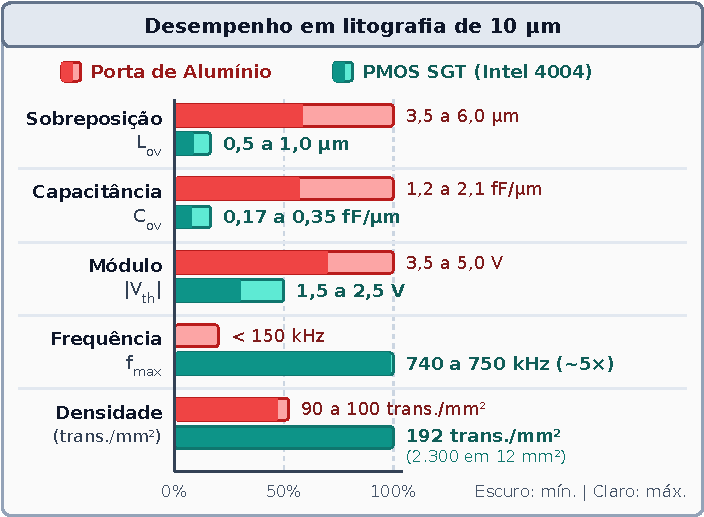
\includegraphics[width=\columnwidth]{desempenho_sgt_10um.pdf}
\caption{Comparação proporcional entre a porta metálica de alumínio e o processo PMOS SGT do Intel 4004 na mesma litografia de \SI{10}{\micro\meter} ($L_{ov}$, $C_{ov}$, $|V_{th}|$, frequência $f_{max}$ e densidade de transistores).}
\label{fig:desempenho_sgt_10um}
\end{figure}

\begin{table*}[!t]
\renewcommand{\arraystretch}{1.2}
\caption{Comparativo Tecnológico Quantitativo entre Porta de Alumínio e Tecnologia SGT}
\label{tab:comparativo_sgt}
\centering
\begin{tabularx}{\textwidth}{>{\raggedright\arraybackslash}p{3.4cm} >{\raggedright\arraybackslash}p{3.8cm} >{\raggedright\arraybackslash}p{4.1cm} >{\raggedright\arraybackslash}X}
\toprule
\textbf{Parâmetro Técnico} & \textbf{Processo PMOS com Porta de Alumínio} & \textbf{Processo PMOS SGT (Intel 4004)} & \textbf{Fundamento Físico e Referência} \\
\midrule
Tolerância de alinhamento ($\Delta L_{align}$) & \SIrange{3}{5}{\micro\meter} & \SI{0}{\micro\meter} (autoalinhado) & Porta de polissilício atua como máscara de difusão (\cref{eq:lov_sgt}) \cite{kerwin1969patent, faggin1970}. \\
Comprimento de sobreposição ($L_{ov}$) & \SIrange{3,5}{6,0}{\micro\meter} & \SIrange{0,5}{1,0}{\micro\meter} & Sobreposição restrita à difusão lateral sob o óxido (\cref{eq:lov_sgt}) \cite{faggin1970}. \\
Capacitância de sobreposição ($C_{ov}$) & \SIrange{1,2}{2,1}{\femto\farad\per\micro\meter} de canal & \SIrange{0,17}{0,35}{\femto\farad\per\micro\meter} de canal & Redução de 60\% a 80\% com $C_{ox} \approx \SI{0,345}{\femto\farad\per\micro\meter\squared}$ (\cref{eq:cov}). \\
Efeito Miller dinâmico ($C_{in,Miller}$) & $(4\text{ a }6) \times C_{gd,metal}$ & $(4\text{ a }6) \times C_{gd,SGT}$ & Amplificação por $(1 + |A_v|)$ sobre $C_{gd}$ três a cinco vezes menor (\cref{eq:miller}) \cite{sze2006}. \\
Tensão de alimentação ($V_{DD}$) & \SIrange{-24}{-28}{\volt} & \SI{15}{\volt} entre trilhos ($V_{SS} - V_{DD}$) & Operação com $V_{SS} = \SI{+5}{\volt}$ e $V_{DD} = \SI{-10}{\volt}$ após redução de $|V_{th}|$ \cite{intel1971datasheet}. \\
Interface com circuitos TTL & Incompatível diretamente, exige conversores & Compatível em nível alto pelo trilho de \SI{+5}{\volt} & Eliminação de tradutores externos com lógica bipolar \cite{intel1971datasheet}. \\
Frequência máxima de relógio & Inferior a \SI{150}{\kilo\hertz} & \SIrange{740}{750}{\kilo\hertz} (\SI{740,7}{\kilo\hertz} nominal) & Ganho de velocidade de até cinco vezes em litografia de \SI{10}{\micro\meter} (\cref{eq:res_fmax}) \cite{faggin1996}. \\
Camadas condutoras de roteamento & Camada única de alumínio & Duas camadas isoladas (polissilício e alumínio) & Roteamento ortogonal duplo elimina túneis difusos \cite{vadasz1972patent, faggin2021}. \\
Densidade bruta de integração & \numrange{90}{100} transistores por \si{\milli\meter\squared} & \num{192} transistores por \si{\milli\meter\squared} (\num{2300} em \SI{12}{\milli\meter\squared}) & Compactação por contatos enterrados e duas camadas condutoras (\cref{eq:res_densidade_int}) \cite{faggin2018howwemade}. \\
Corrente de fuga e estabilidade & Suscetível a desvios iônicos e \textit{spiking} & Fuga mais de 100 vezes menor e limiar estável & Recozimento refratário com captura iônica em $\text{POCl}_3$ \cite{faggin1970}. \\
\bottomrule
\end{tabularx}
\end{table*}

\begin{table*}[!t]
\renewcommand{\arraystretch}{1.2}
\caption{Inovações Técnicas de Faggin no Intel 4004, Mecanismos Físicos e Desdobramentos Industriais}
\label{tab:inovacoes_faggin}
\centering
\begin{tabularx}{\textwidth}{>{\raggedright\arraybackslash}p{4.0cm} >{\raggedright\arraybackslash}p{5.5cm} >{\raggedright\arraybackslash}X}
\toprule
\textbf{Inovação Técnica e Período} & \textbf{Mecanismo Físico ou Arquitetural} & \textbf{Desdobramentos Industriais} \\
\midrule
Porta autoalinhada de silício (SGT, 1968 a 1970) & Porta de polissilício $p^+$ como máscara de difusão térmica e controle de carga interfacial (\cref{eq:lov_sgt,eq:vth_expandido,eq:delta_phims}). & Estreia fabril no Fairchild 3708, adoção na DRAM Intel 1103 e base para a velocidade de operação do 4004 \cite{faggin1970}. \\
Contato enterrado (\textit{Buried Contact}, 1968 a 1970) & Junção ôhmica direta entre polissilício e difusão sem vias para o alumínio, reduzindo a área das células lógicas. & Compactação da pastilha para \SI{3}{\milli\meter} por \SI{4}{\milli\meter}, evitando áreas superiores a \SI{20}{\milli\meter\squared} e preservando o rendimento \cite{vadasz1972patent, faggin2021}. \\
Carga ativa com \textit{bootstrapping} dinâmico (1970 a 1971) & Acoplamento capacitivo em nó flutuante (\cref{eq:delta_vg_boot,eq:vg_total_boot}) mantendo $|V_{GS}| > |V_{th}|$ durante a descarga. & Restauração da excursão plena $V_{out} = V_{DD}$ e ampliação das margens de ruído nos barramentos internos \cite{faggin1996}. \\
Roteamento ortogonal em lógica aleatória (1970 a 1971) & Pistas verticais de polissilício e horizontais de alumínio em duas camadas isoladas, ligadas por vias e contatos enterrados. & Execução do traçado manual da CPU sem ferramentas automáticas, base do projeto VLSI estruturado \cite{mead1980, faggin2021}. \\
Barramento multiplexado em DIP de 16 pinos (1970 a 1971) & Compartilhamento temporal de 4 pinos bidirecionais de dados e controle em oito subciclos (A1 a X3) por instrução. & Viabilização do encapsulamento cerâmico padrão de 16 pinos e operação sincronizada da família MCS-4 \cite{intel1971datasheet, faggin1974patent}. \\
\bottomrule
\end{tabularx}
\end{table*}

\subsection{Impactos na Indústria e na Sociedade}
\label{subsec:impactos_sociedade}

A disponibilidade comercial do Intel 4004 reestruturou o projeto de equipamentos digitais ao substituir a lógica discreta cabeada, formada por circuitos cuja função fica fixada permanentemente nas ligações físicas entre portas lógicas separadas e fios soldados em placa, por arquiteturas programáveis em memória \cite{faggin1972fourchip, cavin2012}. Até o início da década de 1970, desenvolver um controlador exigia interligar dezenas de encapsulamentos TTL SSI e MSI em placas dedicadas. Qualquer ajuste funcional obrigava redesenhar placas e matrizes fabris, gerando elevados custos de engenharia não recorrente (NRE, sigla para o gasto inicial único com projeto, máscaras e ferramental antes da produção em série) e prazos de vários meses. Com o conjunto MCS-4 (CPU 4004, ROM 4001, RAM 4002 e registrador 4003), uma placa substituiu em média noventa chips TTL discretos, transferindo a lógica do produto para o \textit{firmware}, isto é, o programa de baixo nível gravado em memória não volátil para governar o hardware (\cref{fig:impacto_ssi_vs_mcs4}) \cite{faggin1996, intel1988annualreport}. Alterações passaram a ocorrer pela regravação do código em máscaras de ROM ou em memórias EPROM (memórias somente de leitura programáveis e apagáveis por luz ultravioleta, próprias para testes e atualizações rápidas), comprimindo o ciclo de desenvolvimento de meses para semanas e reduzindo custos de manufatura e manutenção \cite{faggin1972fourchip, intel1988annualreport}.

\begin{figure}[!t]
\centering
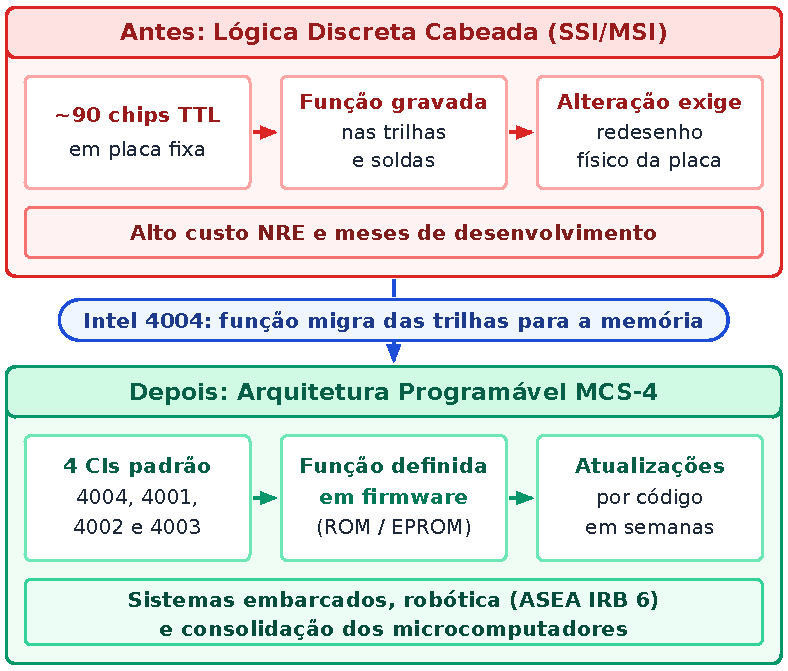
\includegraphics[width=\columnwidth]{impacto_ssi_vs_mcs4.pdf}
\caption{Transição estrutural promovida pelo conjunto MCS-4: substituição de dezenas de circuitos TTL em lógica discreta cabeada por quatro componentes padronizados cuja função reside no \textit{firmware} armazenado em ROM ou EPROM.}
\label{fig:impacto_ssi_vs_mcs4}
\end{figure}

Essa programabilidade consolidou os sistemas embarcados, computadores dedicados incorporados ao interior de máquinas e equipamentos para executar tarefas específicas de controle. Após estrear na calculadora impressora Busicom 141-PF em 1971, a família MCS-4 avançou sobre segmentos antes atendidos por mecanismos eletromecânicos \cite{chm2007panel, intel1988annualreport}. Na instrumentação biomédica, o analisador clínico de eletroforese (técnica laboratorial que separa proteínas em amostras biológicas mediante campo elétrico) da Helena Laboratories substituiu múltiplas placas dedicadas e uma fonte por um módulo compacto com o Intel 4004, reduzindo o volume físico e o custo de produção do equipamento \cite{intel1988annualreport}. O novo modelo também equipou balanças comerciais com cálculo automático de preço por peso, controladores adaptativos de semáforos, bombas de combustível automatizadas e caixas registradoras. No setor de máquinas recreativas operadas por moedas, o protótipo de pinball \textit{Flicker} (1974), desenvolvido pela Dave Nutting Associates com base no Intel 4004, antecipou as mesas comerciais em estado sólido, termo que designa a eletrônica de semicondutores sem peças mecânicas nem relés. Esse protótipo permanece distinto do posterior modelo comercial \textit{Spirit of 76} da Mirco Games, que adotou o Motorola 6800 \cite{faggin1996, faggin2021, intel1988annualreport}.

Na automação fabril e na robótica, a arquitetura derivada do 4004 viabilizou o controle programável de manipuladores industriais. Em 1974, o robô sueco ASEA IRB 6 estreou como o primeiro manipulador industrial totalmente elétrico comandado por microprocessador, utilizando o Intel 8008, herdeiro direto da metodologia SGT consolidada no 4004. Ao substituir relés eletromecânicos, contadores analógicos e longos chicotes de fiação por controle digital, o sistema elevou o tempo médio entre falhas (MTBF, intervalo médio de operação contínua antes de uma pane reparável) e aumentou a precisão de repetição.

A difusão fabril desses controladores programáveis também alterou a composição do emprego industrial. O estudo de Sar A. Levitan e Clifford M. Johnson, publicado em 1982 na revista \textit{Monthly Labor Review} do Bureau of Labor Statistics, documentou que a adoção de microprocessadores e robôs não provocou desemprego estrutural súbito e generalizado, isto é, perda duradoura de vagas por obsolescência tecnológica de ocupações inteiras, mas desencadeou uma redistribuição gradual de postos de trabalho \cite{bls1982futurework}. A demanda por tarefas manuais repetitivas retraiu-se enquanto cresceram as funções ligadas à programação, manutenção eletrônica e supervisão digital. Essa tendência foi corroborada por estudos econômicos sobre máquinas CNC (máquinas-ferramenta de comando numérico computadorizado, cujos movimentos de corte são guiados por programas digitais em vez de ajustes manuais), cujas instalações registraram maior produtividade acompanhada de maior exigência de qualificação técnica \cite{nber2022cnc}.

A metodologia do Intel 4004 alicerçou ainda a linhagem de microprocessadores de 8 bits conduzida por Faggin na década de 1970, representada na \cref{fig:linhagem_faggin_cpu}. Em 1972, o Intel 8008 empregou o mesmo processo PMOS SGT de \SI{10}{\micro\meter} com \num{3500} transistores e endereçamento de até 16 quilobytes \cite{faggin1996}. Em 1974, Faggin e Masatoshi Shima lideraram o Intel 8080 em tecnologia NMOS SGT de \SI{6}{\micro\meter} a \SI{2}{\mega\hertz}, integrando endereçamento de 64 quilobytes e pilha de execução externa (estrutura na memória RAM que armazena endereços de retorno de sub-rotinas sem se limitar a registradores internos fixos), viabilizando o computador Altair 8800 em 1975 \cite{noyce1981}. Em 1976, já na Zilog, Faggin e Shima lançaram o Z80 com circuito de refrescamento para DRAM (lógica embutida que renova periodicamente a carga das células capacitivas da memória dinâmica para evitar perda de dados) e alimentação unipolar (operação com fonte única de \SI{+5}{\volt}, dispensando trilhos negativos adicionais), tornando o Z80 a base para sistemas com o CP/M, sistema operacional padrão dos primeiros microcomputadores de 8 bits antes do MS-DOS \cite{chmz80panel2007}. Em contraste, o processador MOS 6502, criado em 1975 por Chuck Peddle a partir do Motorola 6800, seguiu um ramo arquitetural independente, ilustrando uma trajetória paralela na expansão da computação pessoal, sem vínculo direto com a linhagem SGT iniciada no 4004.

\begin{figure}[!t]
\centering
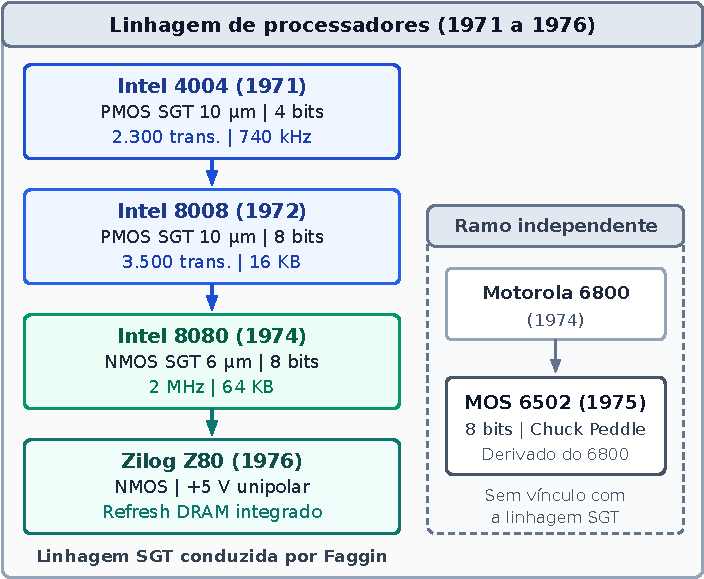
\includegraphics[width=\columnwidth]{linhagem_faggin_cpu.pdf}
\caption{Linhagem arquitetural e de processo do Intel 4004 ao Zilog Z80 (1971 a 1976), destacando o MOS 6502 (1975) como ramo independente derivado do Motorola 6800.}
\label{fig:linhagem_faggin_cpu}
\end{figure}


% % Seção V: Discussão (Física e arquitetura, economia e limites do PMOS)
% % ==============================================================================
% secoes/05_discussao.tex - SEÇÃO V: DISCUSSÃO
% Tema: Federico Faggin e o Primeiro Microprocessador Monolítico (Intel 4004)
% ==============================================================================

\section{Discussão}
\label{sec:discussao}

Os resultados apresentados nas seções anteriores elucidam que o surgimento do primeiro microprocessador monolítico decorreu da convergência coordenada entre física do estado sólido, microarquitetura computacional e viabilidade manufatureira. Longe de representar um desdobramento isolado da engenharia de software ou da teoria lógica, o Intel 4004 corporificou uma reestruturação profunda na cadeia de suprimentos da microeletrônica, transformando a dinâmica de desenvolvimento de sistemas digitais. A análise histórica e tecnológica demanda examinar detalhadamente as restrições físicas dos dispositivos semicondutores, as forças econômicas que reorientaram o mercado internacional e os paralelos historiográficos com iniciativas contemporâneas no início da década de 1970.

\subsection{Engenharia de Dispositivos versus Arquitetura Lógica}
\label{subsec:dispositivos_vs_arquitetura}

A historiografia convencional da computação com frequência separa a formulação arquitetural de alto nível da engenharia de dispositivos em nível de semicondutores. Sob essa ótica dicotômica, a concepção de uma unidade central de processamento seria tratada prioritariamente como um problema de decomposição funcional, definição de repertório de instruções e transferência entre registradores. Contudo, o projeto do MCS-4 demonstrou que a viabilidade prática de uma arquitetura integrada dependia de forma incondicional das propriedades físicas e geométricas dos transistores fabricados no silício \cite{cavin2012}. Sem um alinhamento rigoroso entre a microarquitetura e o processo de fabricação, as propostas conceituais mais elegantes permaneciam confinadas a diagramas teóricos.

A contraproposta de Hoff e Mazor de substituir os circuitos dedicados da calculadora Busicom por uma arquitetura programável de quatro componentes permaneceu como especificação funcional abstrata por mais de seis meses \cite{faggin1996}. Sua execução em tecnologia PMOS de porta de alumínio era inviável: as tolerâncias litográficas inflavam a capacitância Miller, limitando a frequência a patamares inferiores a \SI{150}{\kilo\hertz} e impedindo o cumprimento do ciclo de \SI{10.8}{\micro\second}, enquanto o roteamento em camada única com túneis difusos exigiria mais de \SI{20}{\milli\meter\squared} de área, inviabilizando o rendimento fabril. Faggin superou esse bloqueio ao integrar o SGT com contatos enterrados, \textit{bootstrapping} dinâmico e roteamento ortogonal duplo, viabilizando a CPU em \SI{12}{\milli\meter\squared} a \SI{740}{\kilo\hertz} \cite{faggin1970, faggin2021}.

\subsection{Reorganização Econômica da Indústria de Semicondutores}
\label{subsec:reorganizacao_economica}

O lançamento comercial do Intel 4004 provocou uma profunda reconfiguração nos modelos de negócios e na economia de manufatura de componentes eletrônicos. Até então, a produção de circuitos integrados complexos (LSI) subordinava-se ao modelo de circuitos sob encomenda dedicada, em que cada cliente financiava o leiaute exclusivo para sua aplicação específica. Esse paradigma impunha elevados custos de engenharia não recorrente, prazos de entrega dilatados e riscos comerciais elevados para as fundições de semicondutores. A chegada do microprocessador quebrou esse modelo ao introduzir componentes programáveis de uso geral produzidos como itens de catálogo (\textit{standard parts}) em larga escala \cite{faggin1972fourchip}.

A transição para processadores de catálogo ativou poderosas economias de escala na indústria eletrônica. A fabricação em massa de pastilhas idênticas permitiu acelerar a curva de aprendizado nas linhas de difusão e fotolitografia, reduzindo os custos médios unitários e aumentando a confiabilidade fabril. Os volumosos investimentos em pesquisa, desenvolvimento e leiaute físico puderam ser diluídos entre centenas de clientes e diversas aplicações industriais, desde instrumentos de pesagem e bombas de combustível até caixas registradoras e terminais bancários. A diferenciação funcional do produto final deixou de residir na topologia física dos transistores gravados no silício e foi transferida integralmente para o programa armazenado na memória ROM ou nas memórias reprogramáveis EPROM.

Essa migração do valor agregado acelerou a desverticalização estrutural do setor de computadores e sistemas de controle. Empresas fabricantes de equipamentos deixaram de necessitar de investimentos intensivos em fundições proprietárias de semicondutores, concentrando seus esforços na especificação de sistemas e no desenvolvimento de software. Por sua vez, a padronização do hardware fomentou o nascimento de um segmento independente voltado a ferramentas de apoio à programação, abrangendo montadores, simuladores, compiladores e emuladores em tempo de execução. O microprocessador monolítico estabeleceu desse modo o ecossistema fundacional para os sistemas embarcados e viabilizou a descentralização do poder computacional em escala planetária.

\subsection{Restrições Físicas da Tecnologia PMOS e a Transição Tecnológica}
\label{subsec:limitacoes_pmos_nmos}

Apesar da consolidação prática do Intel 4004, a tecnologia PMOS SGT utilizada em sua fabricação apresentava limites físicos intrínsecos que restringiam o avanço do desempenho. A principal restrição residia na assimetria de mobilidade dos portadores de carga no silício semicondutor. As lacunas no canal PMOS exibem mobilidade típica situada entre \SIrange{150}{200}{\centi\meter\squared\per\volt\per\second}, valor quase três vezes inferior à mobilidade dos elétrons, que varia entre \SIrange{500}{800}{\centi\meter\squared\per\volt\per\second} \cite{sze2006}. Essa desvantagem física forçava o dimensionamento de transistores com largura de canal expressivamente maior para fornecer a mesma corrente de dreno, elevando a capacitância geométrica intrínseca e penalizando a velocidade de chaveamento.

Adicionalmente, a lógica PMOS com transistores de carga ativos apresentava dissipação contínua de potência estática no estado condutivo, limitando o número total de componentes integráveis no encapsulamento antes do alcance de limites térmicos destrutivos. As tensões de polarização eram igualmente complexas e assimétricas, demandando fontes de alimentação externas de \SI{+5}{\volt} e \SI{-10}{\volt} para garantir compatibilidade nos níveis lógicos com a família TTL. Essas condicionantes motivaram a liderança técnica de Faggin e Masatoshi Shima a conduzir a transição para a tecnologia NMOS SGT de \SI{6}{\micro\meter}, culminando no desenvolvimento do processador Intel 8080 em 1974 \cite{faggin1996,chmz80panel2007}. Ao utilizar elétrons como portadores majoritários, o 8080 alcançou frequência de operação de \SI{2}{\mega\hertz}, barramento de dados de 8 bits, endereçamento de \SI{64}{\kilo\byte} com ponteiro de pilha na memória RAM e compatibilidade unipolar plena com níveis TTL a \SI{5}{\volt}.

A evolução subsequente da microeletrônica encontrou seu vetor definitivo na adoção generalizada da lógica complementar CMOS, teorizada e sistematizada por Carver Mead e Lynn Conway \cite{mead1980,weste2010}. Ao combinar transistores nMOS e pMOS em pares complementares, a tecnologia CMOS anulou a corrente de repouso entre a alimentação e a terra, confinando a dissipação de potência quase que exclusivamente aos instantes de comutação lógica. Esse princípio físico sustentou a viabilidade do modelo analítico formulado por Robert Dennard e seus colaboradores na IBM \cite{dennard1974}. O escalamento de Dennard estabeleceu que, ao miniaturizar as dimensões físicas dos transistores e as tensões de alimentação segundo um fator constante, a densidade de integração aumentava quadraticamente e a velocidade crescia linearmente sem elevar a densidade de potência dissipada, fornecendo a base física para a trajetória decenal descrita pela Lei de Moore \cite{moore1965}.

\subsection{Confronto Historiográfico e Limitações do Estudo}
\label{subsec:confronto_historiografico}

A consolidação histórica da precedência do Intel 4004 exige uma contextualização técnica rigorosa diante de projetos concorrentes desenvolvidos no mesmo período. Entre esses projetos destaca-se o circuito TMS 1000 desenvolvido por Gary Boone e Michael Cochran na Texas Instruments \cite{boone1973patent,boone1978patent}. Fabricado em tecnologia PMOS de porta metálica convencional, o TMS 1000 integrou em uma única pastilha a unidade de processamento de 4 bits, memória ROM de programa de um quilobyte, memória RAM estática de 256 bits e portas paralelas de entrada e saída. Em termos funcionais, o TMS 1000 constituiu o primeiro microcontrolador em pastilha única voltado a controle dedicado de baixo custo com programa pré-gravado em máscara, enquanto o Intel 4004 foi concebido e implementado como uma unidade central de processamento flexível com barramento de expansão externa para sistemas gerais de computação.

Outro marco contemporâneo relevante foi o circuito AL1 concebido por Lee Boysel na Four-Phase Systems \cite{boysel1970}. O AL1 consistia em um circuito integrado LSI de 8 bits que reunia registradores de armazenamento e uma unidade lógica e aritmética construída com tecnologia MOS de porta de alumínio e controle de quatro fases. Não obstante seu elevado grau de integração, o AL1 não incorporava uma unidade autônoma de controle sequencial, decodificação de instruções ou manipulação de barramento externo, funcionando como um fatiador aritmético (\textit{bit-slice}). No minicomputador System IV/70, três circuitos AL1 operavam em paralelo subordinados a múltiplos chips externos que realizavam o controle de microcódigo, a geração de pulsos de relógio e o controle de memória.

De forma análoga, o projeto militar Central Air Data Computer (CADC) desenvolvido por Ray Holt e Steve Geller na Garrett AiResearch para o caça Grumman F-14 Tomcat representou uma complexa realização técnica entre 1968 e 1970 \cite{holt1998cadc}. O CADC MP944 era um chipset multichip composto por seis circuitos LSI de 20 bits fabricados pela American Microsystems sob processo PMOS de porta metálica, projetado para o processamento numérico de equações aerodinâmicas de voo em tempo real. Apesar da sofisticação de sua arquitetura paralela com ponto fixo fracionário, o conjunto MP944 operava como um agrupamento multichip com lógica especializada, permanecendo sob estrito sigilo militar até 1998 e, portanto, sem influência direta na evolução do mercado de microprocessadores civis de uso geral.

Por fim, cabe registrar as delimitações metodológicas que balizam o presente estudo. A investigação concentrou-se prioritariamente na linhagem tecnológica trilhada por Federico Faggin nas passagens pela Fairchild, Intel e Zilog, bem como no domínio da tecnologia de transistores de efeito de campo MOS. Dessa forma, o trabalho não analisa exaustivamente a influência concorrente das famílias lógicas bipolares de altíssima velocidade, como ECL e TTL Schottky, que dominaram o segmento de minicomputadores e computadores de grande porte na mesma época. Ademais, as deduções contrafactuais referentes ao atraso de propagação e rendimento da porta metálica de alumínio baseiam-se em modelos analíticos de primeira ordem e regras clássicas de escalamento físico, constituindo inferências de engenharia solidamente fundamentadas na literatura e não medições empíricas sobre réplicas físicas reais.

% % Seção VI: Conclusão
% % ==============================================================================
% secoes/06_conclusao.tex - SEÇÃO VI: CONCLUSÃO
% Tema: Federico Faggin e o Primeiro Microprocessador Monolítico (Intel 4004)
% ==============================================================================

\section{Conclusão}
\label{sec:conclusao}

O Intel 4004 superou a tirania dos números (\cref{eq:tirania_numeros}), segundo a qual a confiabilidade cai conforme cresce a quantidade de componentes interligados, e atendeu à previsão de Moore ao reunir funções aritméticas, lógicas e de controle em uma única pastilha de silício \cite{morton1958, moore1965}. Essa consolidação eliminou centenas de conexões externas entre módulos discretos que elevavam o custo de montagem e a taxa de falhas dos computadores. A análise reunida nas \cref{sec:fundamentacao,sec:resultados} comprova que arquiteturas lógicas só se tornam fabricáveis quando integradas à física de dispositivos e ao \textit{layout}. Ao substituir a porta metálica de alumínio pelo eletrodo de silício policristalino na tecnologia de porta autoalinhada (SGT), o processo contornou os limites capacitivos e de tensão de limiar dos transistores PMOS anteriores \cite{faggin1970}. Sobre essa base tecnológica, as soluções implementadas por Federico Faggin e sintetizadas na \cref{tab:inovacoes_faggin}, centradas nos contatos enterrados, no \textit{bootstrapping} dinâmico e no roteamento ortogonal em duas camadas, levaram a CPU à produção comercial \cite{faggin1996, faggin2021}.

No plano industrial e econômico, o conjunto MCS-4 consolidou a transição dos circuitos dedicados sob encomenda, precursores dos modernos ASICs (\textit{Application-Specific Integrated Circuits}, chips projetados para uma única função fixa), para componentes programáveis de catálogo apoiados em memórias de leitura (ROM e EPROM) e de acesso aleatório (RAM) (\cref{subsec:reorganizacao_economica}) \cite{faggin1972fourchip}. Ao transferir a lógica dos produtos de ligações físicas rígidas para instruções gravadas em memória, esse modelo reduziu os custos iniciais de projeto e consolidou os sistemas embarcados no controle de equipamentos médicos, comerciais e industriais. A partir dessa herança técnica, os processadores de 8 bits Intel 8008, Intel 8080 e Zilog Z80 impulsionaram a automação fabril, ilustrada pelo robô elétrico ASEA IRB 6, e abriram caminho para a primeira geração da microcomputação pessoal (\cref{subsec:impactos_sociedade}) \cite{noyce1981, chmz80panel2007, bls1982futurework}.

Na trajetória física posterior dos semicondutores, as restrições de velocidade e dissipação dos transistores PMOS orientaram a passagem para o processo NMOS, baseado em elétrons mais velozes, e depois para a lógica complementar CMOS, que reduziu o consumo em repouso e sustentou o escalamento proporcional de Dennard por mais de três décadas (\cref{subsec:limitacoes_pmos_nmos,fig:transicao_mos_dennard}) \cite{dennard1974, mead1980}. Quando a miniaturização geométrica atingiu a barreira de potência (limite de calor dissipado por área) e esbarrou em efeitos quânticos (vazamento de elétrons através de isolantes ultrafinos por tunelamento), o encolhimento isolado dos transistores deixou de gerar ganhos proporcionais de desempenho \cite{cavin2012}. Diante dessas barreiras físicas, a adoção da co-otimização entre projeto e tecnologia (DTCO, \textit{Design-Technology Co-Optimization}, prática em que físicos de materiais, engenheiros de fábrica e arquitetos projetam em conjunto desde o início) reafirma a atualidade do método integrado aplicado por Faggin no Intel 4004.


% ------------------------------------------------------------------------------
% ELEMENTOS PÓS-TEXTUAIS (BIBLIOGRAFIA IEEE)
% ------------------------------------------------------------------------------
\bibliographystyle{IEEEtran}
\bibliography{pos_textuais/01_referencias}

\end{document}
